
Ley de Exponentes
\vspace{-5cm}
\LnxPregunta{ \quad Ley de exponentes  }{ 
		\centering
		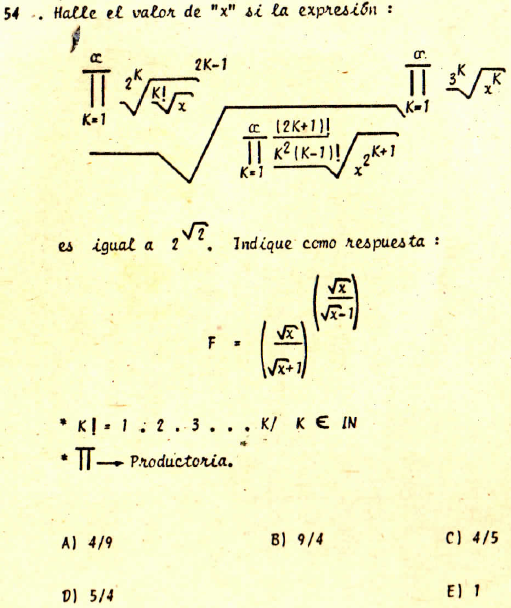
\includegraphics[width=0.95\linewidth]{algebra_pre/Pro_001.png} 
}

 

\LnxSolucion{Solución}{
	
	Sea 
	$$
	\sqrt[\beta]{\theta}^{\alpha} = 2^{\sqrt{2}}
	$$
	donde $\alpha, \beta$ y $\theta$ son:
	\begin{equation*}
		\scalebox{0.95}{$\displaystyle
			\alpha=\prod_{k= 1}^{\infty} \sqrt[3^k]{x^k}, \quad  \beta = \prod_{k=1}^\infty \left( \sqrt[2^k]{ \sqrt[k!]{x} } \right)^{2k - 1}, \quad \theta = \prod_{k=1}^\infty  \sqrt[\frac{(2k+1)!}{k^2 \cdot (k-1)!} \;\;\; ]{ \displaystyle x^{2^{k+1}}} 
			$} 
	\end{equation*} 
	Calculamos $\alpha$, [{\small(La demostración de la convergencia queda como ejercicio para el lector)}]
	$$
	\alpha=\prod_{k= 1}^{\infty} \sqrt[3^k]{x^k} = (x)^{\sum_{k=1}^{\infty} k\cdot 3^{-k}}
	$$
Por la serie geométrica  para \(|u| < 1\),
\begin{equation*}
	\scalebox{0.8}{$\displaystyle
		\sum_{k=1}^\infty k u^k = u \bqty{\dv{u}(\sum_{k=0}^\infty u^k) } = u \bqty{\dv{u}(\frac{1}{1 - u}) }     
		= \frac{u}{(1 - u)^2}
		$} 
\end{equation*} 
$$
\rightarrow \alpha  =  (x)^{\sum_{k=1}^{\infty} k\cdot 3^{-k}}= (x)^{\frac{ 1/3}{(1-1/3)^2 } } = x^{3/4}
$$

Calculamos $\beta$, [{\small(La demostración de la convergencia queda como ejercicio para el lector)}]
$$
\beta = \prod_{k=1}^\infty \left( \sqrt[2^k]{ \sqrt[k!]{x} } \right)^{2k - 1} = x ^{ \sum_{k=1}^{\infty} \frac{2k-1}{2^k \cdot k!}}
$$
Calculando  el exponente  $\sum_{k=1}^{\infty} \frac{2k - 1}{2^k \cdot k!}$, 
 
\begin{align*}
	\sum_{k=1}^{\infty} \frac{2k - 1}{2^k \cdot k!}
	&= \sum_{k=1}^\infty \frac{1}{2^{k-1} \cdot (k-1)!} - \sum_{k=1}^\infty \frac{1}{2^k \cdot k!} \\
	&= \sum_{k=0}^\infty \frac{1}{2^k \cdot k!} - \sum_{k=1}^\infty \frac{1}{2^k \cdot k!}  = 1
\end{align*}
$$
\Rightarrow \beta =x^{1}=x
$$
Calculamos $\theta$, [{\small(La demostración de la convergencia queda como ejercicio para el lector)}]
\[
\theta = \prod_{k=1}^\infty  \sqrt[\frac{(2k+1)!}{k^2 \cdot (k-1)!} \;\;\; ]{ \displaystyle x^{2^{k+1}}}  = (x)^{\sum_{k=1}^\infty \frac{2^{k+1}\cdot k^2 \cdot (k-1)!}{ (2k+1)!}}
\]
Calculando  el exponente  $ \sum_{k=1}^\infty \frac{2^{k+1}\cdot k^2 \cdot (k-1)!}{ (2k+1)!}$, 
\begin{align*}  
	\sum_{k=1}^\infty \frac{2^{k+1}\cdot k  \cdot (k )!}{ (2k+1)!} &=\frac{1}{2}\bqty{   \sum_{k=1}^\infty \frac{2^{k}  \cdot (k-1 )!}{ (2k-1)!}- \frac{2^{k+1}\cdot   (k )!}{ (2k+1)!}}\\
	&=\frac{1}{2}\pqty{2+\sum_{k=1}^\infty \frac{2^{k+1}\cdot   (k )!}{ (2k+1)!} - \sum_{k=1}^\infty \frac{2^{k+1}\cdot   (k )!}{ (2k+1)!} }=1
\end{align*}
$$
\rightarrow \theta = x ^1 = x
$$
Entonces, reemplazando $\alpha, \beta $ y $\theta$:
$$
\sqrt[\beta]{\theta}^{\alpha} =\sqrt[x]{x}^{x^{3/4}} = x^{x^{-1/4}} =2^{\sqrt{2}}
$$
Elevamos a $(-1/4)$
$$
\pqty{x^{-1/4}}^{\pqty{ x^{-1/4}}} = \pqty{2^{\sqrt{2}} }^{-1/4}= \pqty{\frac{1}{2}}^{\frac{\sqrt{2}}{4}}= \pqty{\frac{1}{\sqrt{2}}}^{\pqty{\frac{1}{\sqrt{2}}}}
$$
$$
x^{-1/4} = \frac{1}{\sqrt{2}} \Rightarrow x^{1/4} = \sqrt{2} \Rightarrow x = (\sqrt{2})^4 = 4
$$

Finalmente, reemplazamos $x$ en $F$,
 }

\begin{LnxRptaBox}
	\[
	F= \pqty{\frac{\sqrt{x}}{\sqrt{x}+1}}^{\pqty{\frac{\sqrt{x}}{\sqrt{x}-1}}} = \pqty{\frac{2}{3}}^{\frac{2}{1}}= \frac{4}{9}
	\]
\end{LnxRptaBox}
